\documentclass[10pt,twocolumn]{article}

\usepackage[letterpaper,margin=0.72in,columnsep=0.25in]{geometry}
\usepackage[T1]{fontenc}
\usepackage[utf8]{inputenc}
\usepackage{lmodern}
\usepackage{microtype}
\usepackage{amsmath,amssymb}
\usepackage{booktabs}
\usepackage{enumitem}
\usepackage{xspace}
\usepackage{xcolor}
\usepackage{graphicx}
\usepackage{tikz}
\usepackage{natbib}
\usepackage{hyperref}
\usepackage{balance}

\usetikzlibrary{arrows.meta,positioning,fit,shapes.geometric}

\definecolor{fusionblue}{HTML}{3157D5}
\definecolor{fusionink}{HTML}{172033}
\definecolor{fusiongray}{HTML}{687386}
\definecolor{fusionorange}{HTML}{B85B00}

\hypersetup{
  colorlinks=true,
  linkcolor=fusionblue,
  citecolor=fusionblue,
  urlcolor=fusionblue,
  pdftitle={Fusion: Allocating Intelligence Across Heterogeneous Language Models}
}

\setlist{nosep,leftmargin=*}
\setlength{\parindent}{0pt}
\setlength{\parskip}{0.45em}
\newcommand{\systemname}{\textsc{Fusion}\xspace}
\newcommand{\evidencepending}[1]{\textcolor{fusionorange}{\textbf{[Evidence pending:} #1\textbf{]}}}
\newcommand{\principle}[1]{\begin{quote}\color{fusionink}\itshape #1\end{quote}}

\title{\vspace{-1.6em}\textbf{Fusion: Allocating Intelligence Across\\Heterogeneous Language Models}\\[0.35em]
\large Uncertainty-Directed Orchestration for a New Scaling Dimension}
\author{Fusion Research Team}
\date{Draft --- August 2026}

\begin{document}
\maketitle

\begin{abstract}
Progress in language-model systems is usually measured along a single axis: the
capability of the strongest model available. At inference time, systems often
extend that axis by multiplying calls to similarly capable frontier models.
We argue for a complementary scaling dimension: \emph{allocation intelligence},
the ability to determine what decision-relevant evidence is missing, which
model--role computation can supply it, and when further computation is no
longer worth its cost. We present \systemname, a compound model system that
organizes computation around uncertainty rather than around a fixed model or
agent topology. It maintains one canonical task state, exposes bounded views to
multiple non-authoritative evidence producers, and reserves client-visible
answers and actions for a single authoritative synthesizer. This separation
supports asymmetric model pools, adaptive fan-out, role-conditioned evidence,
and state-aware operation across both one-shot questions and long agentic
workflows. We further describe how task outcomes can train a conditional model
of capability and allocation, allowing system performance to improve both when
underlying models advance and when the system learns to use them better. Our
central objective is not to maximize the number of model calls, but to make
system capability grow faster than its consumption of frontier compute.
\end{abstract}

\section{Introduction}

The supply of machine intelligence is expanding rapidly. Models differ not
only in overall quality, but in scientific knowledge, formal reasoning, code
generation, critique, tool use, latency, and price. Yet most inference systems
still consume this supply through one of two simple patterns. A request is sent
to one general-purpose frontier model, or it is broadcast to several strong
models whose answers are subsequently ranked, voted on, or synthesized.

Both patterns place the model at the center of the system. They ask which model
should answer, or how many answers should be generated. They do not directly
ask the more consequential question: \emph{what is unresolved in the current
task state, and what computation is most likely to resolve it?}

This distinction matters because model calls are not independent units of
intelligence. Two highly capable models may reproduce the same reasoning and
the same error. A smaller specialist may expose a decisive counterexample that
a second frontier model misses. In a long-running workflow, no language model
can determine whether a test passed without observing the environment. And
after enough evidence has accumulated, an additional answer can add cost and
latency without changing the decision.

We introduce \systemname, a model system built around \emph{allocation
intelligence}: the ability to allocate heterogeneous model capability according
to the marginal value of evidence in the current task state. \systemname does
not treat a model output as a vote or an action. It treats each model--role call
as a conditional evidence source and preserves one authoritative path from the
canonical task state to the next response or external action.

This perspective produces a system that is asymmetric by design. Cheap and
specialized models can explore, solve, or critique; programmatic checks and
tools can contribute scoped observations; and a stronger model can retain
decision authority without performing every unit of work itself. Compute
efficiency is therefore not a secondary commercial constraint. It is evidence
that the system can distinguish useful computation from redundant computation.

\paragraph{A new scaling dimension.}
Model progress increases the intelligence available to the system. Allocation
progress increases how effectively that intelligence is converted into task
outcomes. \systemname benefits from both. Our aim is to make system capability
compound faster than frontier-compute consumption, not by weakening the final
decision-maker, but by spending expensive intelligence only where it has high
marginal value.

\paragraph{Contributions.}
This paper makes four claims.
\begin{enumerate}
  \item We formulate multi-model inference as adaptive evidence acquisition
  over a changing task state, rather than as static model selection or answer
  aggregation.
  \item We present a system principle---\emph{one state, many perspectives,
  one commit}---that separates plural evidence generation from singular answer
  and action authority.
  \item We describe an uncertainty-directed architecture that jointly reasons
  about task structure, workflow phase, model capability, evidence readiness,
  cost, and risk.
  \item We define an empirical and learning agenda for allocation intelligence:
  performance--compute frontiers, conditional contribution, long-horizon task
  success, and outcome-driven improvement of the allocation policy.
\end{enumerate}


\section{A New Scaling Dimension}

The dominant story of AI progress is model scaling. Better data, algorithms,
and compute produce more capable models. This remains the primary source of
machine intelligence, and Fusion is designed to benefit from every advance it
creates.

But once multiple capable models exist, a second question becomes unavoidable:
how effectively can a system turn the available supply of intelligence into
useful work?

We call progress in the models themselves \emph{supply-side intelligence
improvement}. We call progress in understanding and satisfying the task's
changing needs \emph{demand-side allocation intelligence}. The two are
complementary:

\begin{equation}
  \text{system progress}
  \quad\longleftarrow\quad
  \underbrace{\text{model progress}}_{\text{supply}}
  \quad\times\quad
  \underbrace{\text{allocation progress}}_{\text{demand}}.
\end{equation}

The expression is not a proposed power law. It captures a strategic shift.
Better models improve the ingredients of the system. Better allocation changes
what the system can make from the same ingredients. A new model can strengthen
Fusion immediately; a better capability map, task representation, or stopping
policy can improve the value extracted from every model already in the pool.

\subsection{Capability without proportional frontier compute}

Inference-time compute is valuable when it changes the quality of a decision.
It is waste when it reproduces evidence the system already has, reasons around
an observation only the environment can provide, or continues after the result
has become stable. A system that cannot tell the difference lacks an important
form of intelligence about its own work.

For this reason, compute efficiency in Fusion is not a purchasing optimization
added after quality. It is a consequence of task understanding. The same
allocation decision determines both whether the system gains a useful
perspective and whether a model call earns its cost. The relevant outcome is a
better performance--compute frontier: greater capability without proportional
growth in scarce frontier computation.

This framing also explains why heterogeneity matters. Different models need
not be interchangeable substitutes. They can be different instruments. A
specialist can contribute a domain-specific observation; an efficient model can
search a broad space; an independent critic can find a counterexample; a
frontier model can integrate evidence and exercise judgment. The purpose is not
to prefer small models or large models. It is to assign each unit of work to
the capability with the highest decision value.

\subsection{Scaling through learning}

Allocation intelligence begins as system design, but it becomes a learning
problem. Every task offers evidence about which model helped, under which role,
given which state, at what cost, and with what downstream outcome. Over time,
Fusion can replace static assumptions about model capability with an empirical
map of conditional contribution. It can learn not only \emph{which} model to
call, but \emph{why}, \emph{when}, and \emph{whether} to call one at all.

\principle{Fusion aims to make system capability compound faster than
frontier-compute consumption.}

\section{The Fusion Design Philosophy}

A system that allocates intelligence cannot be organized primarily around a
catalog of models. Models change too quickly, their strengths are conditional,
and a model name says little about what a particular task needs next. Fusion is
instead organized around the information state of the task.

\principle{Organize computation around uncertainty, not models.}

This is the foundational design principle of Fusion. The system begins with
what is unresolved: a missing fact, an untested assumption, a fragile plan, an
ambiguous preference, an incomplete search, or an unobserved state of the
world. Only then does it ask which computation could resolve that uncertainty.

The principle makes the architecture durable. Models, providers, and tools can
change without changing the object the system is trying to control. A new
capability enters Fusion by demonstrating what uncertainty it can resolve, in
which role, under which conditions. The orchestration layer does not need a
permanent ranking of models; it needs an evolving understanding of their
conditional value.

\subsection{From confidence to decision-relevant uncertainty}

Language models contain useful internal signals about uncertainty. Token
entropy captures uncertainty over expression, while semantic entropy can
better reflect disagreement over meaning
\citep{kuhn2023semantic,farquhar2024semantic}. A compound system must go one
step further. It must care about \emph{decision-relevant uncertainty}: what is
unknown that could change the answer, action, or confidence required to
proceed?

This distinction prevents activity from masquerading as progress. Several
models can agree because they share the same training patterns. Many diverse
answers can be irrelevant to the load-bearing decision. Conversely, one small
piece of external evidence can collapse an entire branch of reasoning.

Fusion therefore treats each potential call as an information acquisition
decision. In practical terms, its value is:

\begin{equation}
  \text{value of a call}
  = \text{expected decision improvement}
  - \text{compute} - \text{latency} - \text{risk}.
\end{equation}

The system does not need a perfect Bayesian model of an open-ended task for
this principle to be useful. It needs structured approximations: what claims
are unresolved, what evidence already exists, which failure modes matter, how
ready the workflow is to act, and which source has historically changed similar
decisions. These approximations can be inspected today and learned from
outcomes over time.

\subsection{Models as conditional sources of evidence}

Under this philosophy, a model is not a scalar score and a call is not a vote.
A model is a conditional source of evidence. Its contribution depends on the
task, role, context, evidence already present, provider surface, and budget.
The same model can be highly valuable as a critic and redundant as a second
solver. A lower-cost model can have high marginal value when it searches a
different region or detects a different class of error. A frontier model can
be indispensable when integration, ambiguity, or stakes demand stronger
judgment.

This view gives cost its proper technical meaning. Cost constrains which
observations can be acquired and how often a system can learn from them. A
model's practical capability is inseparable from the conditions under which it
can be deployed. Understanding cost, latency, reliability, complementarity,
and error correlation is part of understanding the model itself.

\subsection{Plural intelligence, singular authority}

Multiple perspectives create value only if the system remains coherent.
Fusion therefore pairs its information principle with an authority principle:

\principle{One state, many perspectives, one commit.}

The system owns one canonical representation of the task and its history.
Models and tools receive bounded views and return attributed evidence. They do
not independently redefine the task, mutate the shared state, or issue
client-visible actions. One authoritative path integrates the evidence and
commits the next answer or transition.

This separates epistemic plurality from operational plurality. Fusion can
search widely without becoming a swarm of conflicting agents. It can challenge
a plan without creating competing world states. And it can remain compatible
with the simple external contract of one model, even while drawing on a much
richer internal supply of intelligence.

Together, the two principles define Fusion's design philosophy:

\begin{itemize}
  \item acquire computation only against a decision-relevant uncertainty;
  \item interpret outputs as scoped, attributed evidence rather than authority;
  \item preserve one canonical task state across the full workflow; and
  \item stop when further evidence is unlikely to change the commitment.
\end{itemize}

\section{Fusion as a Compound Intelligence System}

Fusion turns its design philosophy into a closed loop: understand the state,
identify the missing evidence, allocate the right capability, integrate the
result, and commit one coherent transition. The loop repeats as the task and
the external world change.

\begin{figure}[H]
\centering
\resizebox{0.97\textwidth}{!}{%
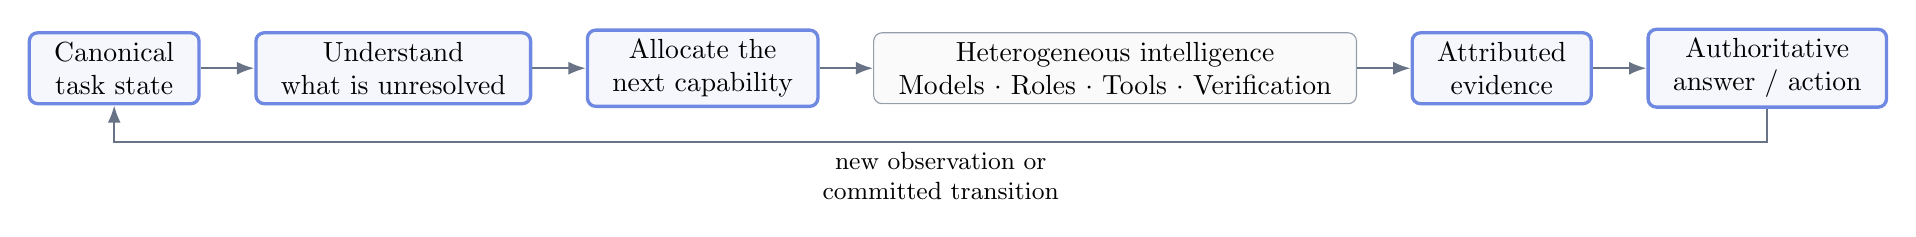
\begin{tikzpicture}[
  node distance=0.68cm,
  box/.style={draw=fusionblue!70, rounded corners=3pt, very thick,
    fill=fusionblue!5, minimum height=0.9cm, align=center, inner xsep=9pt},
  source/.style={draw=fusiongray!70, rounded corners=3pt, fill=black!2,
    minimum height=0.9cm, align=center, inner xsep=9pt},
  arrow/.style={-{Latex[length=2.2mm]}, thick, draw=fusiongray}
]
\node[box] (state) {Canonical\\task state};
\node[box, right=of state] (perceive) {Understand\\what is unresolved};
\node[box, right=of perceive] (allocate) {Allocate the\\next capability};
\node[source, right=of allocate] (sources) {Heterogeneous intelligence\\
  Models $\cdot$ Roles $\cdot$ Tools $\cdot$ Verification};
\node[box, right=of sources] (evidence) {Attributed\\evidence};
\node[box, right=of evidence] (commit) {Authoritative\\answer / action};

\draw[arrow] (state) -- (perceive);
\draw[arrow] (perceive) -- (allocate);
\draw[arrow] (allocate) -- (sources);
\draw[arrow] (sources) -- (evidence);
\draw[arrow] (evidence) -- (commit);
\draw[arrow] (commit.south) -- ++(0,-0.42) -| node[pos=0.25,below,
  font=\small,align=center] {new observation or\\committed transition} (state.south);
\end{tikzpicture}
}
\caption{Fusion continuously matches the changing demand of a task with the
available supply of model and tool intelligence.}
\label{fig:system}
\end{figure}

Five system elements make this possible.

\subsection{A canonical task state}

Fusion begins with one normalized history of the task: the user's intent,
constraints, prior decisions, tool observations, produced artifacts, and
acceptance conditions. This state is more than conversation memory. It is the
reference point against which the system determines what has changed, what is
known, and what remains unresolved.

Different components see purpose-built projections of this state. An explorer
may need the open question without the full interaction history. A critic may
need the candidate and its acceptance criteria. The authoritative synthesizer
retains the native conversation and action contract. Bounded views reduce
irrelevant context and accidental authority while making every contribution
auditable against what its source was allowed to observe.

\subsection{Task and progress understanding}

Fusion distinguishes the structure of a task from the progress of a workflow.
Task understanding identifies the kinds of uncertainty present: alternative
reasoning paths, separable coverage regions, domain knowledge, precision
requirements, external observations, and consequential risks. Progress
understanding asks what can happen next: whether the system needs to discover,
execute, verify, answer, or wait for information only the environment can
provide.

This distinction is critical in long workflows. A difficult task does not
justify maximum computation on every turn. Once an artifact exists, the next
valuable operation may be a deterministic test rather than another proposed
solution. Before a consequential action, an independent critique may be worth
more than additional elaboration. Allocation follows the local state of the
work, not a one-time difficulty label.

\subsection{Adaptive capability allocation}

Given the state, Fusion chooses a source, a role, a context view, and a budget.
It also chooses whether to call anything at all. This policy can vary the
number and type of evidence producers, the strength of the authoritative
synthesizer, the depth of independent audit, and the threshold for stopping.

Roles encode the observation the system wants to acquire, not personas for
generating stylistic variety:

\begin{itemize}
  \item \textbf{Solve} develops an independent candidate when the path is uncertain.
  \item \textbf{Explore} searches for discriminating directions when the space is open.
  \item \textbf{Variant} reveals materially different realizations when criteria or preferences are unresolved.
  \item \textbf{Critique} hunts for counterexamples, hidden risks, and failed conditions.
  \item \textbf{Verify} obtains scoped evidence from tools, tests, or checkable artifacts.
\end{itemize}

Because the value of a model is role- and state-dependent, Fusion can use an
asymmetric portfolio deliberately. Efficient models extend the breadth of
search and audit where their contribution is high. Frontier models concentrate
on integration and decisions that genuinely require their capabilities. The
portfolio is not fixed: either class can be admitted or withheld according to
expected value.

\subsection{Evidence, not votes}

Every contribution enters the system as bounded, attributed evidence. A
candidate solution, a criticism, a test result, and a suggested tool call do
not have the same semantics. Fusion preserves these differences rather than
flattening all outputs into interchangeable answers.

The authoritative synthesizer is therefore not a majority voter. It must judge
which claims are load-bearing, reconcile or reject incompatible evidence, and
satisfy the original client contract. Producer suggestions remain advisory;
only the authoritative path can emit the next answer or external action.

\subsection{Continuity across agentic workflows}

For a one-shot request, the loop ends in an answer. For an agentic workflow, it
ends in one state-consistent transition and then begins again. Fusion preserves
the same authority and evidence semantics through four recurring modes:

\begin{equation}
  \textsc{Discover} \rightarrow \textsc{Execute}
  \rightarrow \textsc{Verify} \rightarrow \textsc{Commit}.
\end{equation}

Discovery finds the observation that best separates live hypotheses. Execution
makes one coherent change. Verification connects recorded evidence to explicit
acceptance conditions. Commitment occurs only when material conditions are
supported. This continuity is what allows Fusion to remain effective beyond a
single response: the allocation decision evolves with the task instead of
being reset at every model call.

\section{Performance Beyond Proportional Compute}
\label{sec:evidence}

The promise of allocation intelligence must be visible from outside the
system. Fusion should not require a customer to choose between frontier-level
capability and practical deployment efficiency. It should move the frontier
itself.

\subsection{A performance--compute frontier across three capability regimes}

Our current evaluation spans scientific reasoning, policy-constrained tool use,
and agentic coding. These workloads expose different failure modes, but ask the
same systems question: how much capability can be delivered for the compute
consumed? Table~\ref{tab:pareto} reports both score and the cost in US dollars
of completing each full benchmark run.

\begin{table}[H]
\centering
\caption{Reported score and full benchmark-run cost. Lower cost and higher
score are better.}
\label{tab:pareto}
\scriptsize
\begin{tabular}{@{}l
  r@{\hspace{1.2em}}r
  @{\hspace{2.0em}}r@{\hspace{1.2em}}r
  @{\hspace{2.0em}}r@{\hspace{1.2em}}r@{}}
\toprule
& \multicolumn{2}{c}{GPQA Diamond}
& \multicolumn{2}{c}{$\tau^3$-Banking}
& \multicolumn{2}{c}{Terminal-Bench v2.1} \\
\cmidrule(lr){2-3}\cmidrule(lr){4-5}\cmidrule(lr){6-7}
System & Score & Cost & Score & Cost & Score & Cost \\
\midrule
\textbf{Fusion Max} & \textbf{94.9\%} & \textbf{13}
  & \textbf{49.5\%} & \textbf{145} & 86.5\% & \textbf{74} \\
GPT 5.6 Sol (max) & 94.1\% & 22 & 44.3\% & 251
  & \textbf{88.0\%} & 86 \\
Claude Fable 5 (fallback) & 92.6\% & 45 & 38.1\% & 322
  & 84.6\% & 299 \\
\addlinespace
\textbf{Fusion Code} & \textbf{93.5\%} & \textbf{7}
  & \textbf{48.5\%} & 159 & \textbf{89.9\%} & 71 \\
Claude Opus 5 (max) & 93.2\% & 18 & 42.1\% & 193
  & 89.1\% & 215 \\
Kimi K3 & \textbf{93.5\%} & 30 & 46.0\% & \textbf{122}
  & 85.0\% & \textbf{56} \\
\bottomrule
\end{tabular}
\end{table}

Fusion Max reduces the aggregate cost of this fixed three-benchmark portfolio
from \$359 to \$232 relative to GPT 5.6 Sol, a 35.4\% reduction. It scores
higher on GPQA Diamond and $\tau^3$-Banking and remains within 1.5 percentage
points on Terminal-Bench. Against Claude Fable 5, Fusion Max scores higher on
all three workloads while reducing each full-run cost by 55--75\%; aggregate
cost falls from \$666 to \$232.

Fusion Code presents a second operating point. It meets or exceeds the reported
score of Claude Opus 5 on all three workloads while reducing full-run cost by
18--67\%; aggregate cost falls from \$426 to \$237. Kimi K3 illustrates a
different trade-off: Fusion Code matches or improves its score on all three
workloads, but spends more on the Banking and Terminal-Bench runs. We therefore
present that comparison as a capability gain, not as a universal cost
reduction.

\evidencepending{before publication, attach immutable run identifiers and
confirm model snapshots, pricing date, task scope, scorer and protocol
versions, attempts and retries, fallback behavior, cache treatment, and the
boundary of included internal usage.}

The result is a Pareto claim, not a discount claim. Fusion retains stronger
judgment where it is valuable and removes the assumption that every
intermediate unit of reasoning must be purchased at the same capability tier.
A system that is only cheaper because it silently accepts worse outcomes has
not demonstrated allocation intelligence.

\subsection{Why asymmetry changes the economics of capability}

The cost profile follows directly from Fusion's architecture. A frontier-heavy
orchestration design assembles its worker pool from several of the most capable
general-purpose models. This can increase quality, but it also duplicates the
most expensive class of computation across planning, generation, critique, and
verification. Fusion instead composes a wider capability spectrum. It asks
where frontier intelligence is decisive and where a specialized or efficient
source can add more information per unit of compute.

Fugu provides a useful external operating point. It uses learned orchestration
across a frontier-heavy worker pool, while Fusion uses task-state understanding
to allocate across an asymmetric supply of models. On the benchmark comparison
available to us, the two systems reach broadly comparable performance, while
Fugu's reported benchmark cost is roughly an order of magnitude higher. The
difference is not incidental pricing. It reflects two system designs: one
primarily orchestrates frontier intelligence; the other learns where frontier
intelligence is necessary.

\evidencepending{insert the audited Fugu case study, with matched task subset,
model and price dates, scaffold differences, attempts, usage boundary, and a
clear distinction between controlled and directional comparisons.}

The point is not that an asymmetric pool is inherently superior. A weak source
that adds misleading or redundant evidence is not efficient at any price
\citep{li2025rethinkingmoa}. The advantage appears only when the system has the
capability understanding and task-state awareness to use asymmetry
selectively. That allocation layer---not the mere presence of smaller
models---is the source of the frontier shift.

\subsection{Effectiveness that survives the workflow}

One-shot benchmarks capture only part of Fusion's value. In an agentic system,
the demand for intelligence changes after every observation and action. A
design that improves a single answer can still fail over a trajectory by
repeating work, losing state, acting on incompatible plans, or declaring
success before verification.

Fusion is designed so that its benefit persists across the workflow. The same
canonical state, uncertainty model, and authority boundary apply whether the
system is investigating, editing, testing, recovering from failure, or
committing a result. The relevant outcome becomes successful task completion,
not the quality of an isolated response. The relevant cost becomes compute per
successful trajectory, not price per API call.

Our long-horizon evaluation therefore measures end-to-end completion, total
cost per success, frontier calls per trajectory, state consistency, recovery
after failed actions, premature completion, and degradation as workflow length
increases. This is where allocation intelligence becomes a system capability
rather than a routing optimization.

\subsection{A transparent standard of evidence}

Public comparisons should expose the full operating point: task set, model and
policy versions, scorer, attempts, timeout, concurrency, cache treatment,
latency, and all internal model usage. Client-visible tokens are not the total
cost of orchestration. Infrastructure and scorer failures must remain separate
from system failures. Fumo Lab will report these boundaries explicitly,
especially where a fast-moving external system cannot be reproduced under a
perfectly matched protocol.

\section{The Compounding Advantage}
\label{sec:learning}

Model progress expands what Fusion can draw upon. Allocation progress determines
how much of that supply becomes useful system capability. The latter is where
Fusion develops its own compounding advantage. An asymmetric model pool can be
copied and a routing graph can be reconstructed; an empirical understanding of
how capabilities interact with real tasks---and a system that improves that
understanding through use---is harder to reproduce.

\subsection{A living map of model capability}

Leaderboards describe average model performance on predetermined tasks. Fusion
needs a different object: a conditional capability map. It asks how likely a
model is to contribute useful evidence for a particular kind of task, under a
particular role, at a particular workflow state, given the evidence already
available.

The map includes capability and operating characteristics together: model and
provider version, task dimensions, role, context, output validity, latency,
cost, observed redundancy, error correlation, synthesizer use, and downstream
outcome. It is versioned because models change. It is uncertainty-aware because
new models and rare tasks begin with limited evidence. And it measures
interaction, because the best standalone answerer is not necessarily the most
valuable next contributor.

This systematic evaluation is what makes heterogeneous allocation reliable.
Without it, asymmetry is merely an intuition that cheaper models might help.
With it, the system can predict where a capability is complementary, where it
is redundant, and where the risk requires escalation.

\subsection{The allocation data flywheel}

Every Fusion task can produce a structured learning record: the state the
system observed, the uncertainty it identified, the call it admitted, the role
and model it selected, the evidence returned, the decision committed, the
resources consumed, and the eventual outcome.

These records improve three layers at once:

\begin{itemize}
  \item \textbf{task understanding}: a richer representation of what real users
  are trying to accomplish and where their workflows become uncertain;
  \item \textbf{capability understanding}: empirical knowledge of what each
  model contributes under real conditions; and
  \item \textbf{allocation policy}: better admission, role assignment,
  escalation, synthesis, and stopping decisions.
\end{itemize}

More use creates a wider view of task demand. Better task understanding creates
better allocation. Better allocation creates more informative observations
about model capability. The result is a flywheel that is grounded not only in
benchmark labels, but in the distribution of real tasks and feedback that the
system encounters.

This flywheel is difficult to reproduce from the surface behavior of Fusion.
It depends on the joint history of tasks, model versions, allocations,
counterfactual probes, and outcomes. The visible architecture is modular; the
accumulated model of conditional contribution is proprietary and compounding.

\subsection{From designed allocation to learned allocation}

Fusion currently combines structured task perception with explicit policy
boundaries. This makes allocation interpretable while the learning base grows.
The same architecture exposes a stable end-to-end learning interface:

\begin{align}
 &(\text{task state},\text{available evidence},\text{model supply}) \notag\\
 &\hspace{2.0em}\longrightarrow
 (\text{next source},\text{role},\text{budget},\text{stop}).
\end{align}

Fumo Lab has begun training models that map user input and evolving task state
directly to allocation decisions. Producer behavior supplies model feedback:
which sources generated novel, valid, or decision-changing evidence.
Synthesizer behavior and downstream outcomes supply system feedback: which
evidence was used, which commitment succeeded, and where the workflow failed.
Together, they create a path toward reinforcement learning from model and
environment feedback for the allocation policy itself.

Learning from production traces requires discipline. The system only observes
the outcomes of calls it chose to make, so naive training would reinforce its
existing blind spots. Controlled exploration, shadow calls, candidate
ablations, offline replay, and local credit assignment are necessary to
estimate what would have happened under another allocation. Privacy,
provenance, evaluation, and rollback must be properties of the learning loop,
not afterthoughts.

\subsection{Bounded system-level recursive improvement}

Fusion improves through two coupled streams. New and better models expand the
supply of intelligence. Better task understanding and allocation extract more
value from that supply. Improvements in either stream change the data available
to the other: stronger producers reveal new possibilities, while a stronger
allocator discovers where each producer matters.

This is recursive improvement in a bounded, system-level sense. Fusion uses
observations of its own decisions and outcomes to improve how future
intelligence is allocated. It does not imply unrestricted self-modification or
an unobservable loop. Policies remain versioned, evaluated, constrained, and
reversible.

\principle{Fusion improves when models improve---and improves again when it
learns how to use them.}

\section{A Broader Shift in AI Systems}

Fusion is part of a broader movement from monolithic model invocation toward
systems that actively shape inference. Routing and cascade systems demonstrate
that quality and cost can be optimized jointly
\citep{chen2023frugalgpt,ong2024routellm,aggarwal2024automix}. Ensembling and
Mixture-of-Agents systems show that multiple candidates can improve a final
answer when their contributions are complementary
\citep{jiang2023llmblender,wang2024moa,lu2026complementary}. Learned
orchestrators increasingly treat worker selection, roles, and topology as
policy decisions
\citep{zhang2025routerr1,yue2025masrouter,nielsen2026conductor,xu2026trinity,fugu2026}.
Long-horizon agents extend the problem from requests to evolving trajectories
\citep{zhang2026mtrouter,koh2026macu}.

Fusion shares the conviction that inference should be adaptive and learnable,
but chooses a broader control object. A router asks which model should answer.
An ensemble asks which answers should be combined. An orchestrator often asks
which worker graph should execute. Fusion asks what decision-relevant evidence
the current task needs next, which capability can provide it, and whether the
system is ready to commit.

That distinction connects several previously separate concerns. Model choice,
role, fan-out, tool use, verification, stopping, cost, and workflow phase all
become aspects of one allocation decision. The conceptual roots include active
information acquisition and value-of-information reasoning
\citep{houlsby2011bald,golovin2011adaptive}; the system contribution is to make
those ideas practical under natural-language ambiguity, correlated model
errors, heterogeneous operating costs, and changing external state.

The important transition is not from one model to many models. It is from
static consumption of intelligence to adaptive allocation of intelligence.

\section{Discussion}

\subsection{What is difficult to copy}

The surface architecture of \systemname is intentionally modular. A capable
synthesizer, several producers, and a router can be reproduced. This is not the
primary moat. The compounding asset is the joint empirical model required to
make the architecture effective:
\begin{itemize}
  \item a versioned capability map over model, role, task, and state;
  \item observed redundancy and error correlation among evidence sources;
  \item a representation of unresolved claims, readiness, and risk;
  \item an allocation and stopping policy trained on task outcomes; and
  \item a dataset connecting orchestration decisions to long-horizon success.
\end{itemize}

More usage can improve each component. Better allocation produces better data
about where models are useful; better data produces better allocation. The
feedback loop is defensible only when outcome attribution, privacy, evaluation,
and rollback are first-class system properties.

\subsection{Why singular authority matters}

Many multi-agent systems treat autonomy as a source of collective capability.
For a model exposed as one API identity, autonomy also creates a consistency
problem. Agents can act from incompatible assumptions, issue duplicate tool
calls, or complete against different interpretations of success. \systemname
separates epistemic plurality from operational plurality: many processes may
search, but one process owns the next externally visible commitment.

This boundary is particularly valuable when the system is embedded inside
another agent. From the caller's perspective, \systemname behaves as one model
with one tool protocol and one conversation state. Internally, it can purchase
as much plural evidence as the decision warrants without exposing a swarm's
coordination burden to the client.

\subsection{Limits of the information-theoretic framing}

The information-acquisition view is a guide, not a claim that natural-language
tasks admit a clean finite hypothesis space. Semantic clusters can be wrong.
Model self-confidence is poorly calibrated. Creative and preference-sensitive
tasks may have no unique latent truth. Evidence sources share data, training
methods, and failure modes that are difficult to observe. The value of a call
can become clear only many steps later.

Consequently, a universal scalar ``uncertainty score'' would be misleading.
Solve, Explore, Variant, and Critique require different state representations
and success signals. Initial policies should remain typed, auditable, and
conservative where actions are consequential. Learned policies should report
calibration and out-of-distribution behavior rather than only average reward.

\subsection{A research agenda for the new scaling dimension}

Three questions determine whether allocation intelligence becomes a durable
scaling dimension.

First, can conditional contribution be predicted well enough to outperform
fixed test-time scaling across changing model pools? Second, can a system learn
to stop without losing rare but consequential corrections? Third, can
trajectory outcomes provide sufficiently local credit to improve allocation
without overfitting to a benchmark or existing policy?

Answering these questions requires scaling experiments, not only endpoint
comparisons. Future evaluations should vary worker capability, pool diversity,
call budget, workflow length, and task distribution. A genuine scaling result
would show that allocation improvements shift the system frontier repeatedly,
not merely at one hand-tuned operating point.


\section{Conclusion}

Fumo Lab's vision is a compound intelligence system whose progress is not
limited to the capability curve of a single model. Fusion advances through two
coupled forces: the model ecosystem supplies stronger and more diverse
intelligence, while the allocation layer learns how to turn that supply into
better outcomes.

The need for this system is becoming more pronounced. Agentic work turns a
request into a trajectory in which the capability and evidence required next
are revealed through execution. At the same time, the model ecosystem is
becoming increasingly heterogeneous. Request-level routing can choose an
answering model, but it cannot fully determine in advance which uncertainty
will become load-bearing as the work unfolds.

Fusion addresses this gap by organizing computation around decision-relevant
uncertainty. It treats models and tools as conditional sources of evidence,
preserves one canonical state, and reserves answers and actions for one
authoritative commitment path. This allows heterogeneous capabilities to
function as one coherent intelligence across both one-shot problems and
long-running workflows.

The immediate result is the possibility of a Pareto improvement: frontier-level
performance with materially lower frontier-compute consumption. The longer-term
result is a system that learns from its own operation. Allocation decisions,
producer behavior, synthesizer use, and downstream outcomes improve the task
representation, capability map, and allocation policy that govern future work.

This is Fusion's bounded form of system-level recursive improvement. Model
progress creates more intelligence; allocation progress determines how much of
it becomes useful; experience improves the allocation of the next task. Fumo
Lab's ambition is to make those forces compound.


\balance
\bibliographystyle{plainnat}
\bibliography{references}
\end{document}
